\documentclass[12pt]{report}

\usepackage[a4paper]{geometry}
%\geometry{left=2.5cm,right=2.5cm,top=2.5cm,bottom=2.5cm, a4paper}
\usepackage[utf8]{inputenc}
\usepackage{amsmath}
\usepackage{amsthm}
\usepackage{amssymb}
\usepackage{ulem}
\usepackage{graphicx}
\usepackage{caption}
\graphicspath{}
\usepackage[document]{ragged2e}
\usepackage{setspace}
\usepackage{tabularx}
\usepackage[slovene]{babel}
\usepackage{textcomp, gensymb}
\usepackage{siunitx}
\usepackage{pdfrender,xcolor}
\usepackage{hyperref}
\usepackage{xurl}
\usepackage{float}
\usepackage{titlesec}

\newfloat{slika}{htbp}{loc}
\floatname{slika}{Slika}

\newfloat{tabela}{htbp}{loc}
\floatname{tabela}{Tabela}

% Differential
\newcommand{\diff}{\mathrm{d}}


\title{
  
\includegraphics[width=0.4\textwidth]{fmf_logo}\\
  {\small Oddelek za fiziko} \\
  {Upogib}\\
  {\small Poročilo pri fizikalnem praktikumu III}\\

}
\date{}
\author{ avtor: Kristofer Č. Povšič \\[5 cm]
 \small  Asistentka: Jelena Vesić
}


\titleformat{\chapter}[hang]{\Huge\bfseries}{\thechapter{. }}{0pt}{\Huge\bfseries}

\setlength\parindent{0pt}

\begin{document}

\setcounter{page}{2}

\maketitle

\chapter*{Uvod}

Lokalne deformacije z napetostjo $\sigma = \frac{F}{S}$ povezuje prožnostni modul $E$ tako, da velja 

\begin{equation}
  \sigma = E \frac{\Delta l}{l}
\end{equation}

kjer je $\frac{\Delta l}{l} = \epsilon$ relativni raztezek/skrček. Ta linearna zveza velja v območju elastičnosti, kjer je relativni raztezek še dovolj majhen. Prožne deformacije materiala preučujemo tako, da palico iz izbranega materiala na koncih podpremo, sredino med podprtima točkama pa obtežujemo s silo uteži. Spodnja stran palice se zaradi natezne sile podaljša, zgornja stran pa se zaradi tlačne sile skrči. Predpostavimo, da je presek palice konstanten. 

Na sredini palice med dvema podprtima točkama velja 

\begin{equation}
  u_0 = \frac{F_0 l^3}{48EJ}
\end{equation}

Zanima nas še maksimalna obremenitev, da lokalne deformacije relativnega raztezka ostanejo pod $0.01\%$. Tako dobimo enačbo 

\begin{equation}
  F_{max} = \frac{8EJ\epsilon}{Dl}
\end{equation}

\chapter*{Naloga}

\begin{enumerate}
  \item Opazuj upogibanje dveh palic različnih presekov v odvisnosti od obremenitve in izračunaj njuna prožnostna modula. 
  \item Oceni maskimalno obremenitev palic ter za koliko se palici upogneta zaradi lastne teže. Primerjaj tudi gostoti obeh palic. 
  \item Nariši diagrama spreminjanja strižne sile in navora vzdolž palice za izbrano utež. 
\end{enumerate}

\begingroup
\let\clearpage\relax

\chapter*{Potrebščine}
\begin{itemize}
  \item stojalo, mikrometrska ura
  \item uteži, tehtnica, kljuka za obešanje uteži 
  \item dve ravni palici okroglega in pravokotnega profila 
  \item kljunasto merilo in meter 
\end{itemize}

\endgroup


\chapter*{Obdelava podatkov}

Meritve koeficienta vzmeti so dale naslednji graf z regresivno premico: 

\begin{slika}[H]
  \centering
  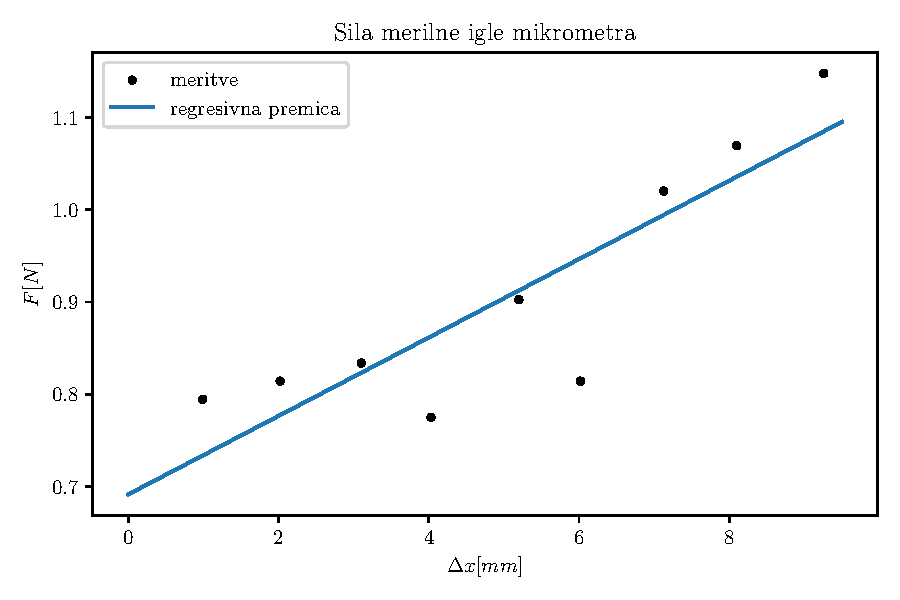
\includegraphics{igla}
  \caption{\small Graf prikazuje silo v odvisnosti od izmerjenega odmika. Z regresivno premico smo dobili koeficient vzmeti mikrometra. Graf ne gre skozi točko (0,0), saj ima igla tudi neko maso.}
\end{slika}

Koeficient vzmeti ima vrednost 

\[
k = (42 \pm 9)  N/m
\]

Izmerimo podatke prve palice s kvadratnim profilom: $m_k = (267 \pm 2)g$, $a = (7.00 \pm 0.02)mm$ in $l = (56.00 \pm 0.02)cm$. 

Gostota palice je 

\[ 
\rho_k = (9730 \pm 90) \frac{kg}{m^3}
\]

\begin{slika}[H]
  \centering
  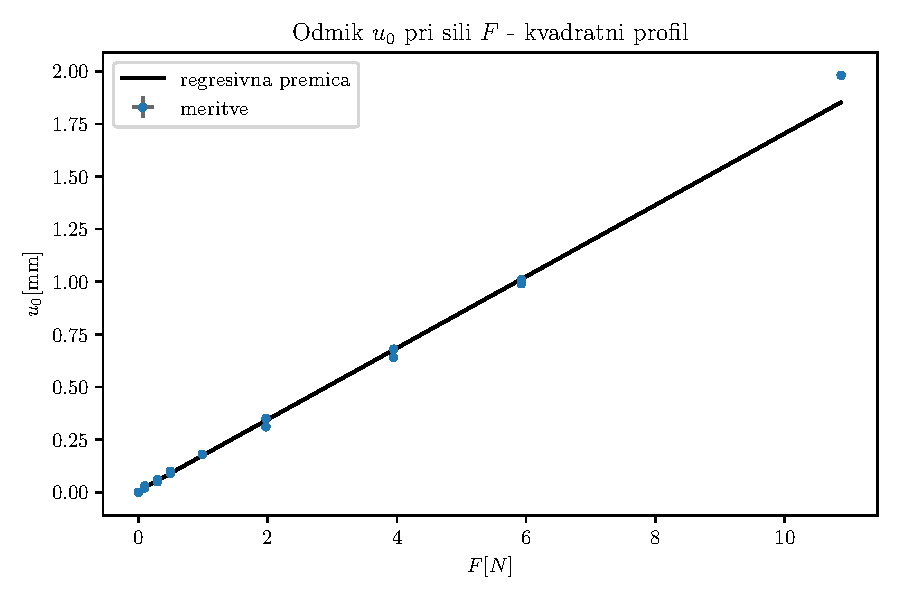
\includegraphics{kvader}
  \caption{\small Graf prikazuje odmik $u_0$ od začetne lege za palico s kvadratnim profilom. }
\end{slika}

Iz tega izračunamo vztrajnostni moment palice in s pomočjo meritev dobimo prožnostni modul materiala palice 

\[ 
E = (108 \pm 2)GPa 
\]

Z dobljenim prožnostnim modulom lahko dobimo tudi maksimalno obtežitev palice, ki znaša 

\[
F_k = (44.0 \pm  0.8)N
\]

Ocenimo še, da se palica zaradi lastne teže povesi

\[
u_g=(0.444 \pm 0.008)mm  
\]

Podatke druge palice z okroglim profilom so: $d = (7.00 \pm 0.02)mm$ in $m_0 = (214 \pm 2)g$. 

Gostota palice tako znaša 

\[
\rho_v = (9900 \pm  100) \frac{kg}{m^3}
\]

Meritve dajo sledeč graf: 

\begin{slika}[H]
  \centering
  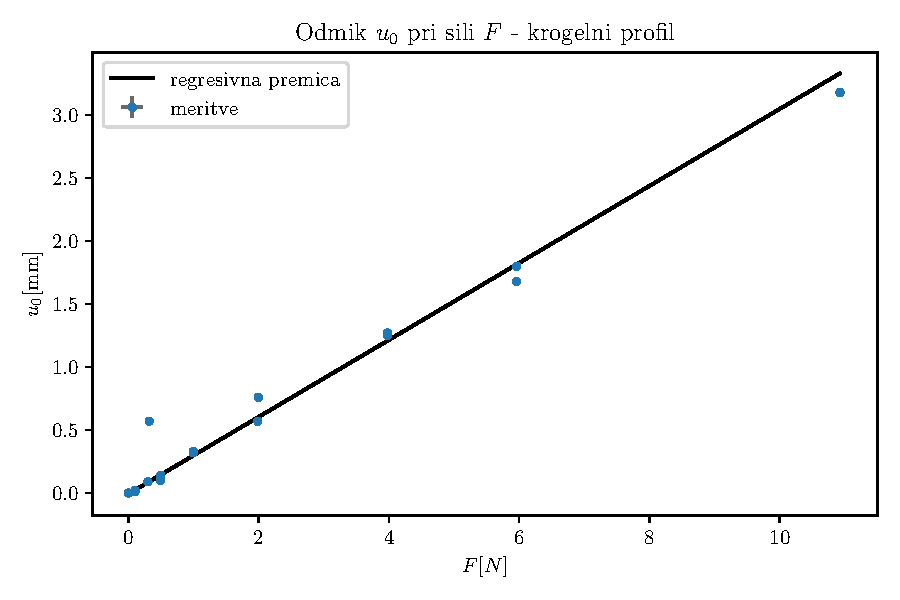
\includegraphics{valj}
  \caption{\small Graf prikazuje odmik $u_0$ od začetne lege za palico z okroglim profilom. }
\end{slika}

Dobimo prožnostnim modul 

\[
E = (102 \pm 8)GPa
\]

maksimalna sila je

\[
F_v = (24 \pm 2)N  
\]

in povesek zaradi lastne teže
\[
u_g = (0.64 \pm  0.05)mm
\]

Vidimo, da se gostoti palici in posledično tudi prožnostna modula znotraj napake ujemata, iz česar lahko predpostavimo, da sta narejenih iz istega/podobnega materiala. 

Za konec narišem še funkcijo $F(x)$ in $M(x)$ po nevtralni ravnini. 

\begin{slika}[H]
  \centering
  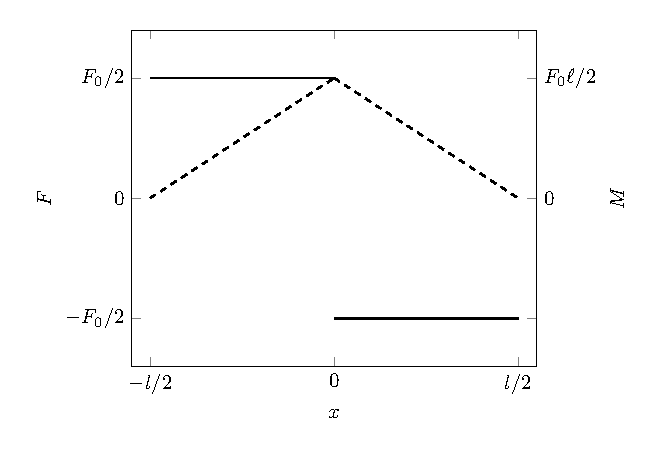
\includegraphics{F-and-M}
\end{slika}

\end{document}